%%%%%%%%%%%%%%%%%%%%%%%%%%%%%%%%%%%%%%%%%
% Beamer Presentation
% LaTeX Template
% Version 1.0 (10/11/12)
%
% This template has been downloaded from:
% http://www.LaTeXTemplates.com
%
% License:
% CC BY-NC-SA 3.0 (http://creativecommons.org/licenses/by-nc-sa/3.0/)
%
%%%%%%%%%%%%%%%%%%%%%%%%%%%%%%%%%%%%%%%%%

%----------------------------------------------------------------------------------------
%	PACKAGES AND THEMES
%----------------------------------------------------------------------------------------
% !TEX TS-program = pdflatexmk
%\makeatletter\let\ifGm@compatii\relax\makeatother
\documentclass[pdftex,12pt,xcolor=pdftex,table]{beamer}
%\documentclass[handout,12pt,xcolor=pdftex,table]{beamer}
\synctex=1
\usepackage{comment}
\usepackage{etex}
\usepackage{amsmath}
\usepackage{amsthm}
\usepackage{amsfonts}
\usepackage{amssymb}
\usepackage{latexsym}
\usepackage{mathtools}
\usepackage[english]{babel}
\usepackage[utf8]{inputenc}
\usepackage{tikz}
\usetikzlibrary{calc,matrix,shapes,arrows}
\usepgflibrary{shapes.arrows}
\usepackage[nomessages]{fp}% http://ctan.org/pkg/fp
\newcounter{mycols}
\usepackage{graphicx} % Allows including images
\usepackage{booktabs} % Allows the use of \toprule, \midrule and \bottomrule in tables
\usepackage[sort]{natbib}
\usepackage{bibentry}
\usepackage{layout}
\usepackage[justification=centering,figureposition=bottom]{caption}
\usepackage{longtable}
\usepackage{lscape}
\usepackage{rotating}
\usepackage[figtopcap,center,scriptsize]{subfigure}%[figtopcap]
\usepackage{appendix}
\usepackage{setspace}
\usepackage[multiple,stable]{footmisc}
\captionsetup[longtable]{width=.75\textwidth}

\mode<presentation> {

% The Beamer class comes with a number of default slide themes
% which change the colors and layouts of slides. Below this is a list
% of all the themes, uncomment each in turn to see what they look like.

%\usetheme{default}
%\usetheme{AnnArbor}
%\usetheme{Antibes}
%\usetheme{Bergen}
%\usetheme{Berkeley}
%\usetheme{Berlin}
%\usetheme{Boadilla}
\usetheme{CambridgeUS}
%\usetheme{Copenhagen}
%\usetheme{Darmstadt}
%\usetheme{Dresden}
%\usetheme{Frankfurt}
%\usetheme{Goettingen}
%\usetheme{Hannover}
%\usetheme{Ilmenau}
%\usetheme{JuanLesPins}
%\usetheme{Luebeck}
%\usetheme{Madrid}
%\usetheme{Malmoe}
%\usetheme{Marburg}
%\usetheme{Montpellier}
%\usetheme{PaloAlto}
%\usetheme{Pittsburgh}
%\usetheme{Rochester}
%\usetheme{Singapore}
%\usetheme{Szeged}
%\usetheme{Warsaw}

% As well as themes, the Beamer class has a number of color themes
% for any slide theme. Uncomment each of these in turn to see how it
% changes the colors of your current slide theme.

%\usecolortheme{albatross}
%\usecolortheme{beaver}
%\usecolortheme{beetle}
%\usecolortheme{crane}
%\usecolortheme{dolphin}
%\usecolortheme{dove}
%\usecolortheme{fly}
%\usecolortheme{lily}
%\usecolortheme{orchid}
%\usecolortheme{rose}
%\usecolortheme{seagull}
%\usecolortheme{seahorse}
%\usecolortheme{whale}
%\usecolortheme{wolverine}

%\setbeamertemplate{footline} % To remove the footer line in all slides uncomment this line
%\setbeamertemplate{footline}[page number] % To replace the footer line in all slides with a simple slide count uncomment this line

%\setbeamertemplate{navigation symbols}{} % To remove the navigation symbols from the bottom of all slides uncomment this line
}

%----------------------------------------------------------------------------------------
%	TITLE PAGE
%----------------------------------------------------------------------------------------

\title[Survival of the richest?]{Survival of the richest? Social status, fertility and social mobility in England 1541-1824} % The short title appears at the bottom of every slide, the full title is only on the title page

\author{Castañeda, M; Padilla, H} % Your name
\institute[PUJ - UA] % Your institution as it will appear on the bottom of every slide, may be shorthand to save space
{
Summer School of Economics: Economic Growth and Comparative Development \\ % Your institution for the title page
\medskip
%\textit{Authors: } % Your email address
}
\date{\today} % Date, can be changed to a custom date

\begin{document}

\begin{frame}
\titlepage % Print the title page as the first slide
\end{frame}

\begin{frame}
\frametitle{Overview} % Table of contents slide, comment this block out to remove it
\tableofcontents % Throughout your presentation, if you choose to use \section{} and \subsection{} commands, these will automatically be printed on this slide as an overview of your presentation
\end{frame}

%----------------------------------------------------------------------------------------
%	PRESENTATION SLIDES
%----------------------------------------------------------------------------------------

%------------------------------------------------
\section{Introduction} % Sections can be created in order to organize your presentation into discrete blocks, all sections and subsections are automatically printed in the table of contents as an overview of the talk
%------------------------------------------------

%\subsection{Research question and motivation} % A subsection can be created just before a set of slides with a common theme to further break down your presentation into chunks

\begin{frame}
\frametitle{Research question and motivation}
 Objective: looks at the role of socio-economic status as a determinant of fertility and social mobility in pre-industrial England.\\~\\

The motivation arises from Clark's main findings about the fertility gap between the rich and the poor and the implications of that on the spread of ‘middle-class values’.\\~\\

Two elements: higher fertility in the richest + rigid social structure  
\end{frame}

%------------------------------------------------


%------------------------------------------------
\section{Data and methodology}
%------------------------------------------------
\begin{frame}
\frametitle{Data description}
 The paper uses the family composition database created by the Cambridge Group. It contains statistics on 26 Anglican parishes in England and covers the period 1541 to 1871.\\~\\
 \begin{figure}[h!]
    \centering
    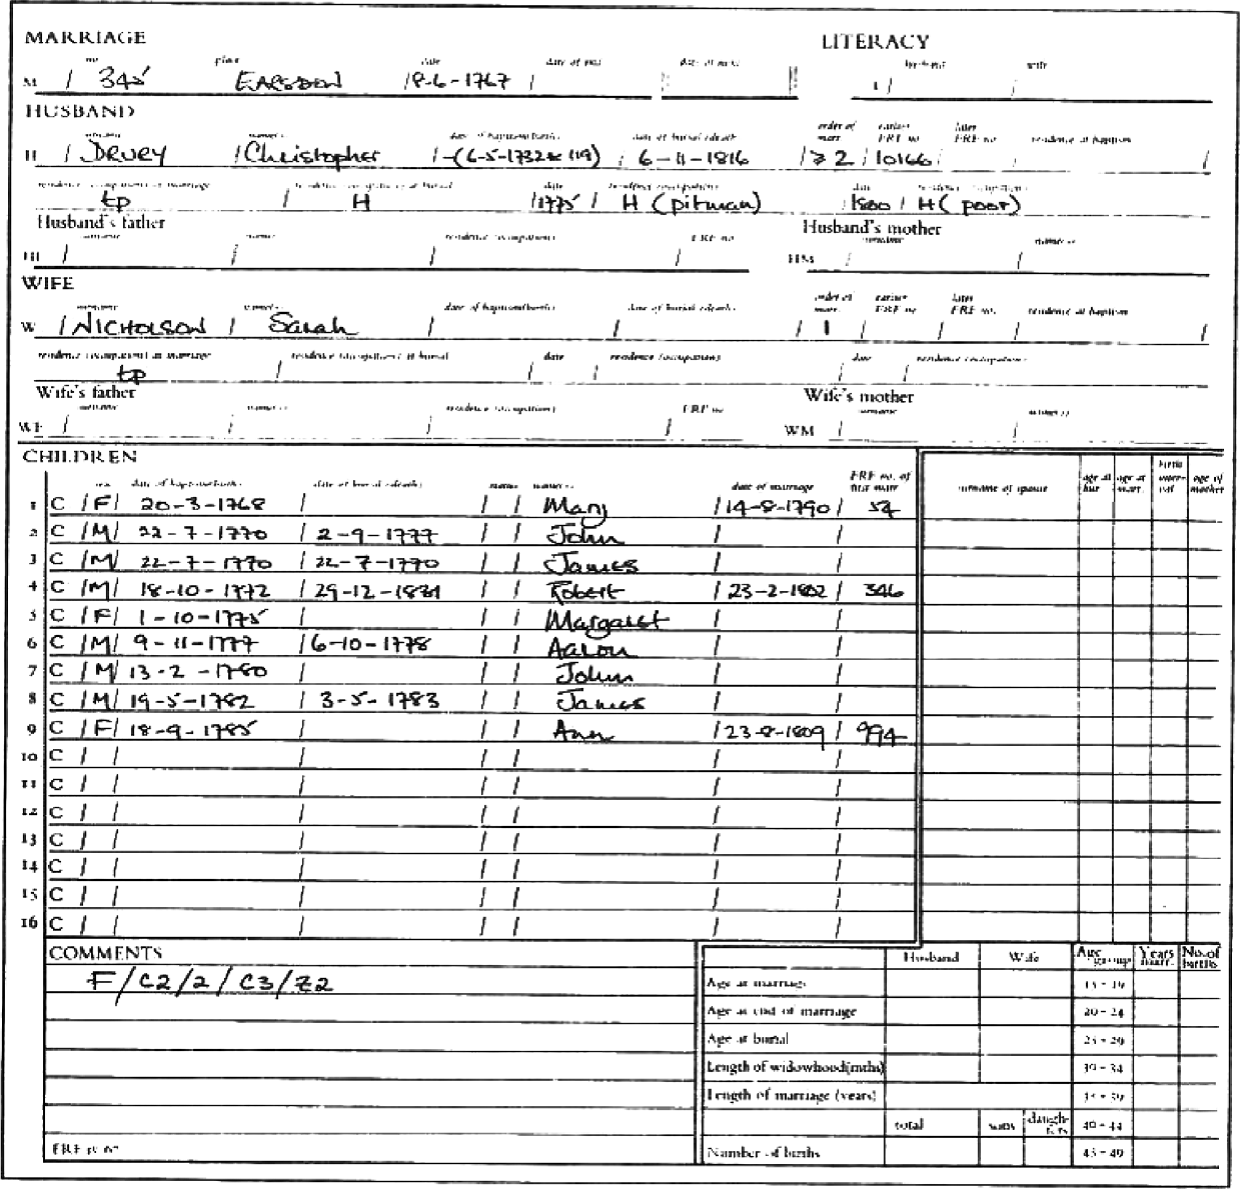
\includegraphics[width=5cm]{formato_constitucion_familia.png}
    \caption{Family reconstitution form}
 \end{figure}

\end{frame}

%------------------------------------------------
\begin{frame}
\frametitle{Data description}
 Each Family Reconstitution Form builds on a unique marriage and includes:\\~\\
 \begin{itemize}
    \item Dates of birth and death of the spouses
    \item Number of offspring
    \item Offspring birth and death dates
    \item Spouses occupations at marriage and at death
  \end{itemize}\\~\\
 If the couple’s offspring themselves went on to marry, then the family reconstitution form will link us to the marriage, and hence a family reconstitution form for the offspring. 

\end{frame}


%------------------------------------------------

\begin{frame}
\frametitle{Data description}
Advantages and disadvantages of the Cambridge Group data against Clark's data:\\~\\

\begin{table}
\begin{tabular}{l l l}
\toprule
\textbf{Advantages} & \textbf{Disadvantages}\\
\midrule
Wide population & No direct information of wealth \\
Larger geographical area & Data missing due to
migration\\
Huge detail of demographic var & Data are mostly
rural \\
\bottomrule
\end{tabular}
\caption{Data comparison}
\end{table}
\end{frame}

%------------------------------------------------
\begin{frame}
\frametitle{Classification of occupations }
Characteristics of the sample
\begin{itemize}
    \item No women include 
    \item Total sample 89,887 but occupation is known for 15,159
    \item Death dates required so the sample is reduced to 9,925 for the fertility analysis 
    \item For the social mobility analysis the son's occupation is required so the sample is reduced to 1,396
    \item Spouses occupations at marriage and at death
  \end{itemize}\\~\\

\end{frame}
%------------------------------------------------
\begin{frame}
\frametitle{Classification of occupations}
The social groups was constructed based on the classification of the occupations carried out by Clark (2010) 
\begin{figure}[H]
    \raggedright
    \centering
    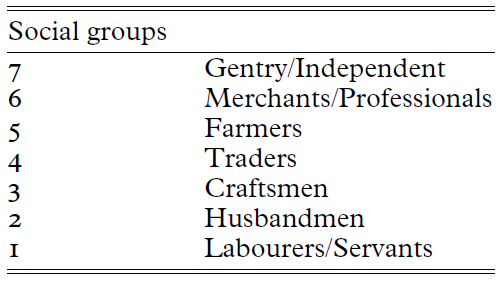
\includegraphics[width=8cm]{table2.PNG}
    \caption{Social groups according to Clark and Cummins (2010)}
 \end{figure}

\end{frame}
%------------------------------------------------
\begin{frame}
\frametitle{Classification of occupations}
The middle class in terms of values and wealth. As to the values, the only variable we can observe is literacy 
\begin{figure}[h!]
    \centering
    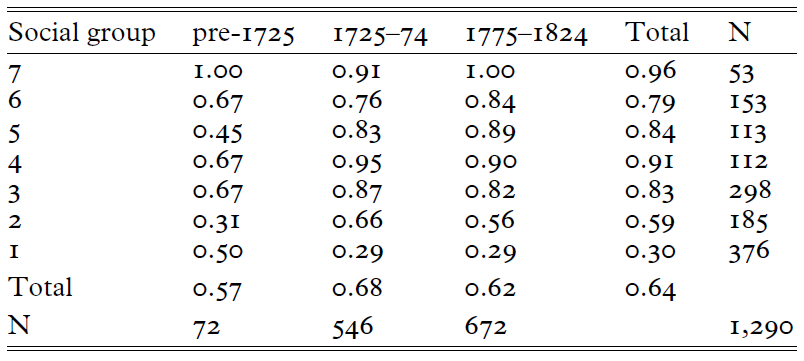
\includegraphics[width=8cm]{table3.PNG}
    \caption{Literacy rate by group}
 \end{figure}

\end{frame}
%------------------------------------------------
\begin{frame}
\frametitle{Empirical strategy} 
Generalized Linear Model: 
\begin{itemize}
    \item Random component: distribution of dependent variable (Negative Binomial) 
    \item Link function (logit)
    \item Systemic Component:  variables specification 
  \end{itemize}\\~\\

\end{frame}

%------------------------------------------------
\section{Results}
%------------------------------------------------
\begin{frame}
\frametitle{Fertility by social group} 
Did wealthier fathers leave more children?
\begin{figure}[h!]
    \centering
    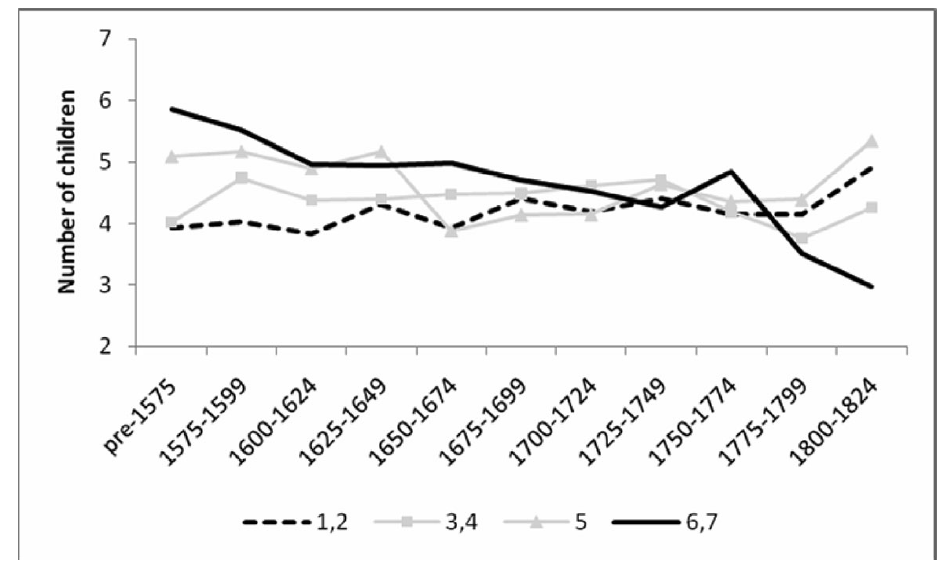
\includegraphics[width=9cm]{figure3.PNG}
    \caption{Fertility by social group}
 \end{figure}
\end{frame}

%------------------------------------------------
\begin{frame}
\frametitle{Fertility by social group} 
What really matters is the the number of children surviving by social class
\begin{figure}[h!]
    \centering
    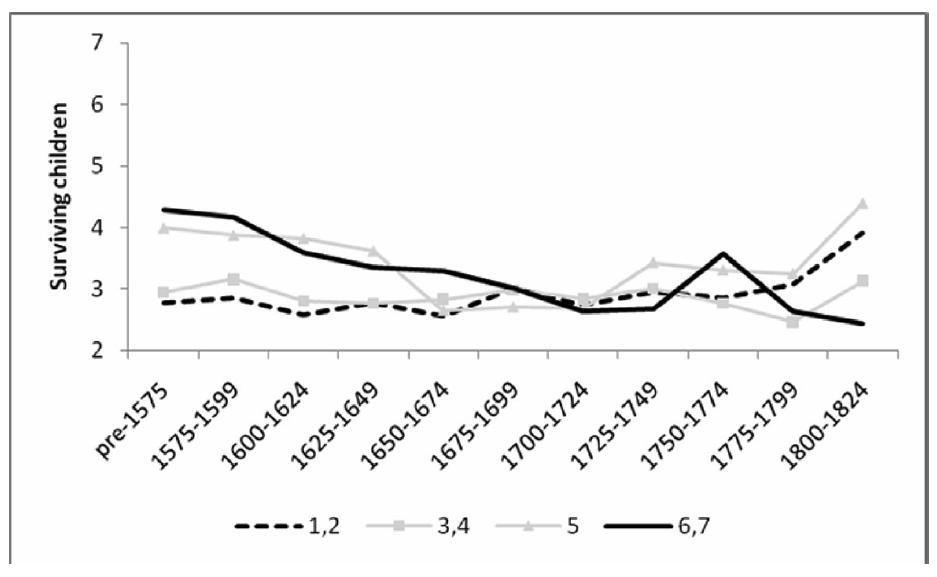
\includegraphics[width=9cm]{figure4.PNG}
    \caption{Reproductive success by social group}
 \end{figure}
\end{frame}

%------------------------------------------------
\begin{frame}
\frametitle{Fertility by social group}
\begin{figure}[h!]
    \centering
    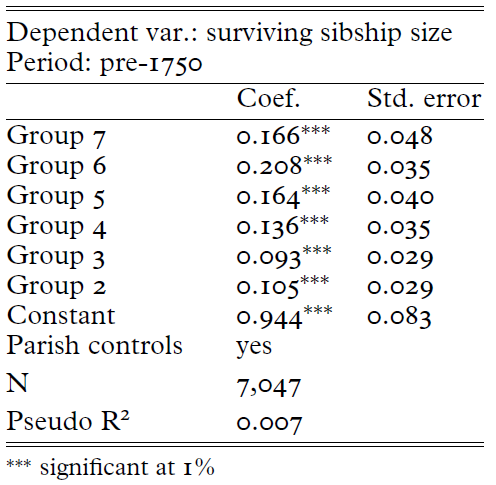
\includegraphics[width=5cm]{table4.PNG}
    \caption{Regressing net fertility on social group for the period until 1750}
 \end{figure}
\end{frame}
%------------------------------------------------
\begin{frame}
\frametitle{Fertility by social group}
\begin{figure}[h!]
    \centering
    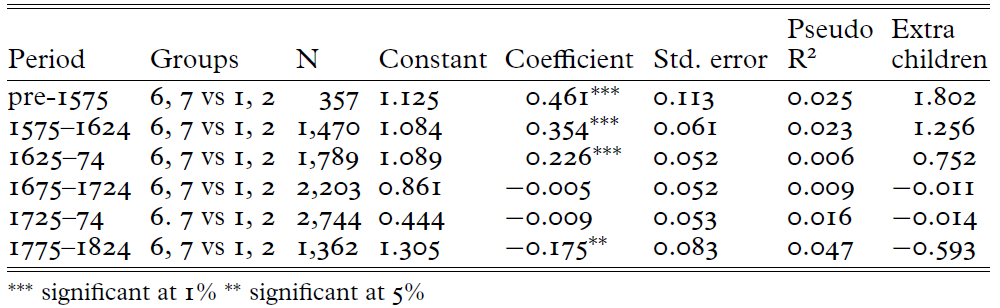
\includegraphics[width=12cm]{table5.PNG}
    \caption{Regressing net fertility on social group by 50-year period}
 \end{figure}
\end{frame}
%------------------------------------------------
\begin{frame}
\frametitle{Fertility by social group}
What explains fertility gaps between classes?\\~\\
    how parents were able to regulate their fertility at a time of limited or no access to contraception\\~\\
    \begin{itemize}
        \item Delaying marriage
        \item Stopping
        \item Spacing 
    \end{itemize}\\~\\
\end{frame}
%------------------------------------------------
\begin{frame}
\frametitle{Fertility by social group}
Delaying marriage: The Rich woman are married first\\~\\
\begin{figure}[h!]
    \centering
    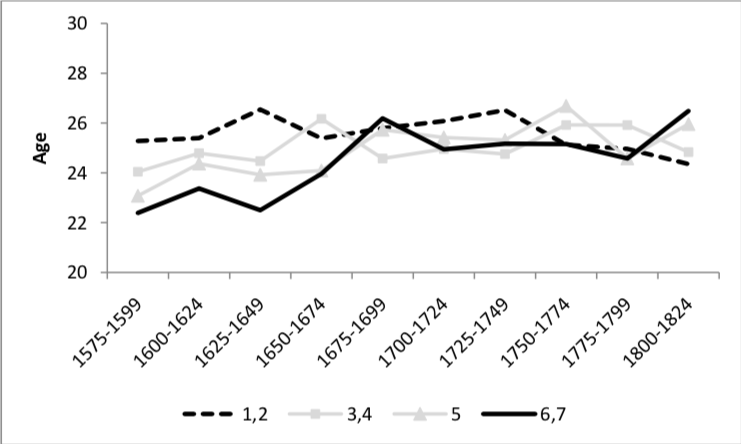
\includegraphics[width=9cm]{figure5.png}
    \caption{Wife's age at first marriage}
 \end{figure}
\end{frame}
%------------------------------------------------
\begin{frame}
\frametitle{Fertility by social group}
Stopping: The decision to stop having children\\~\\
\begin{figure}[h!]
    \centering
    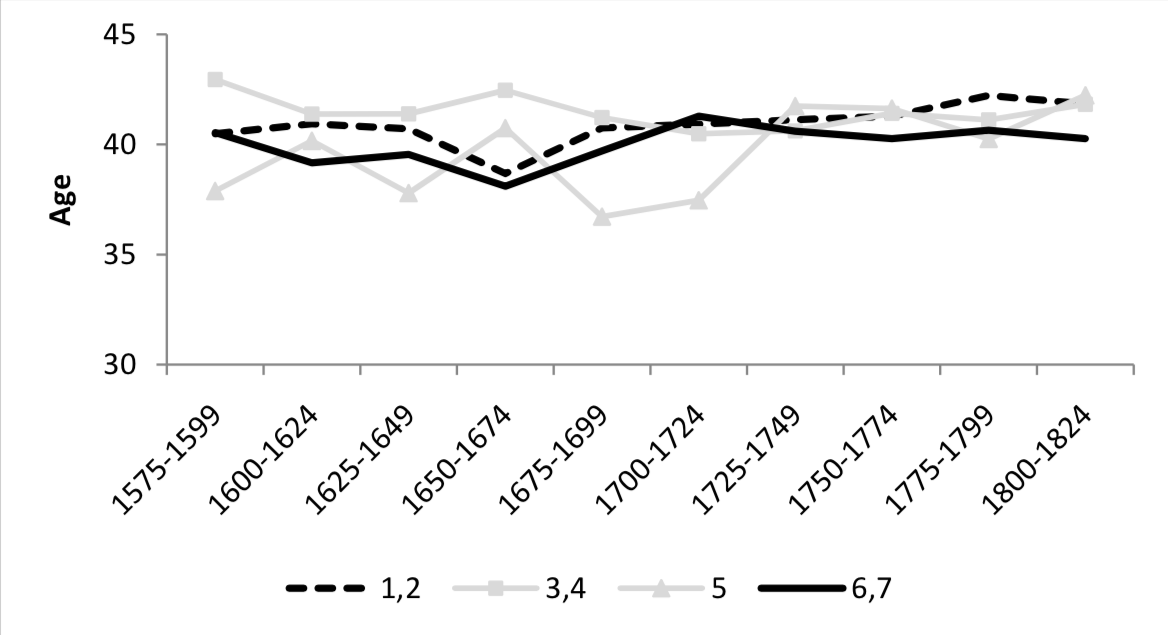
\includegraphics[width=9cm]{figure6.png}
    \caption{Wife's age at last birth marriage}
 \end{figure}
\end{frame}
%------------------------------------------------
\begin{frame}
\frametitle{Fertility by social group}
Spacing: Regulating time intervals between the birth of each child.\\~\\
\begin{figure}[h!]
    \centering
    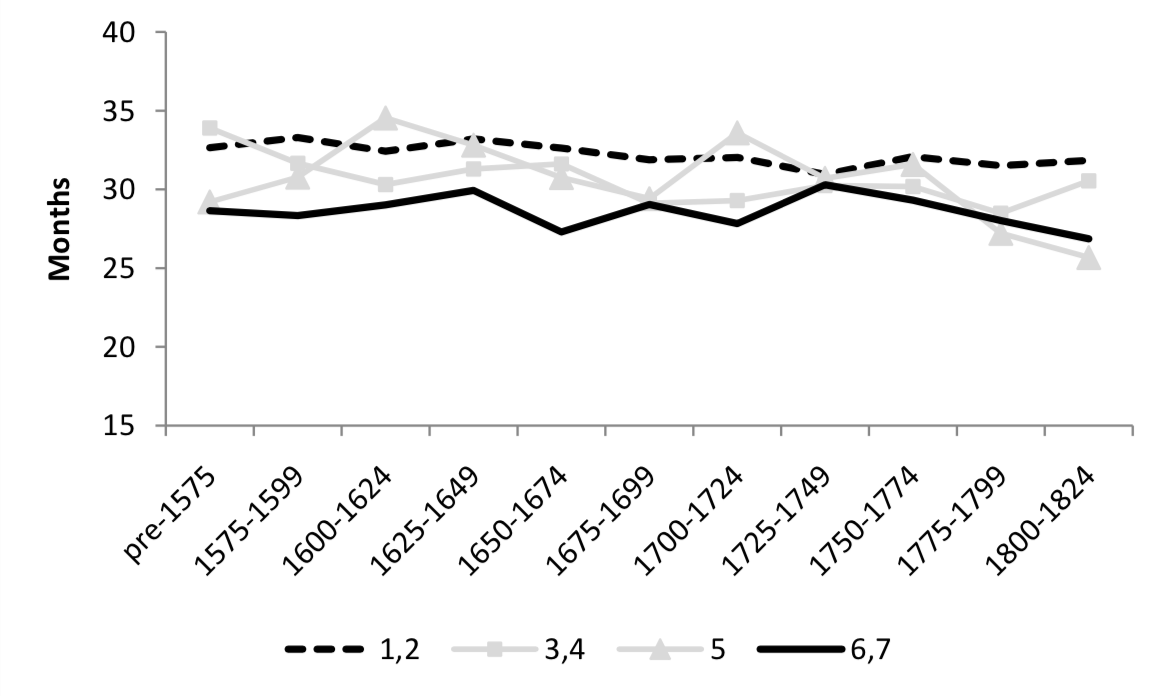
\includegraphics[width=9cm]{figure7.png}
    \caption{Average length of birth interval}
 \end{figure}\\~\\
\end{frame}
%------------------------------------------------
\begin{frame}
\frametitle{Fertility by social group}
The reason that wealthier groups gave birth to more offspring was that less time went by between each birth, and also the fact that they married earlier
\begin{figure}[h!]
    \raggedright   
    \centering
    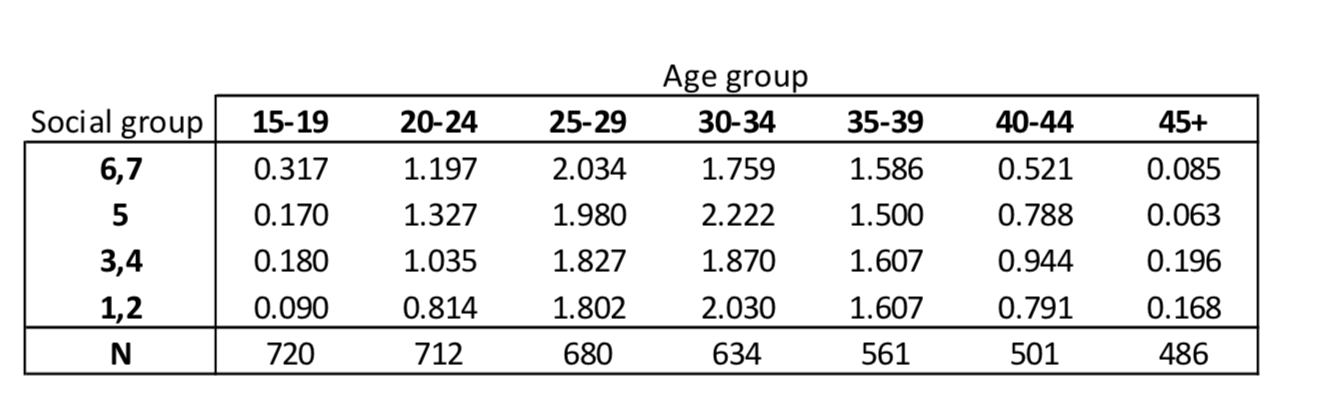
\includegraphics[width=11cm]{table6.png}
    \caption{Average number of children 
    by woman’s age group}
 \end{figure}
\end{frame}
%------------------------------------------------
\begin{frame}
\frametitle{Fertility by social group}
Living conditions and fertility 
\begin{figure}[h!]
    \centering
    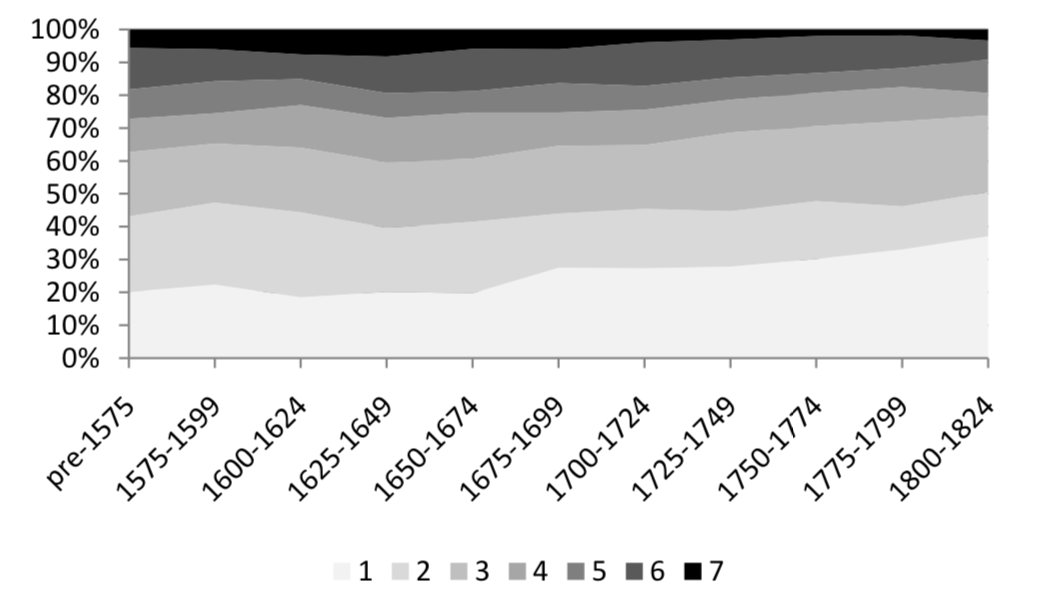
\includegraphics[width=9cm]{figure8.png}
    \caption{Shares of social groups}
 \end{figure}
\end{frame}

%------------------------------------------------
\begin{frame}
\frametitle{Memes or Genes?}
The degree of downward mobility of the higher classes 
\begin{figure}[h!]
    \centering
    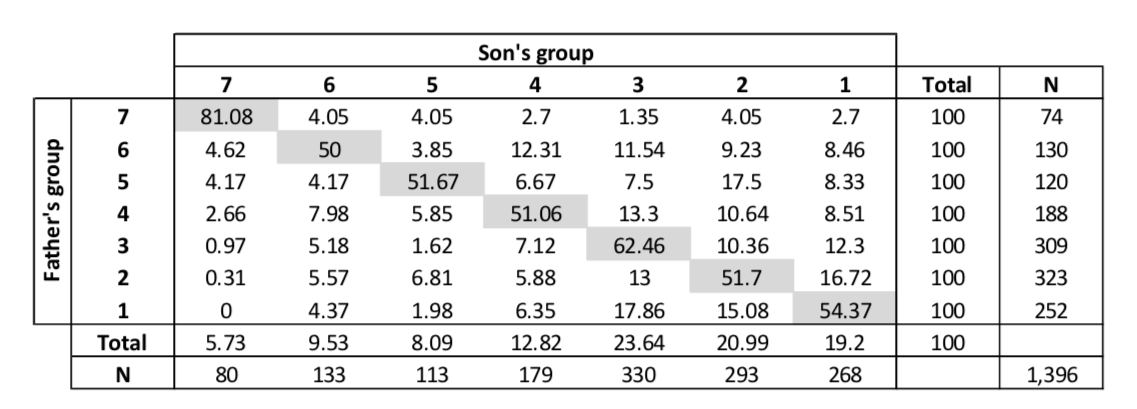
\includegraphics[width=12cm]{table8.png}
    \caption{Outflow mobility, pre‐1750}
 \end{figure}
\end{frame}
%------------------------------------------------
\begin{frame}
\frametitle{Memes or Genes?}
The degree of upward mobility of the lower class
\begin{figure}[h!]
    \centering
    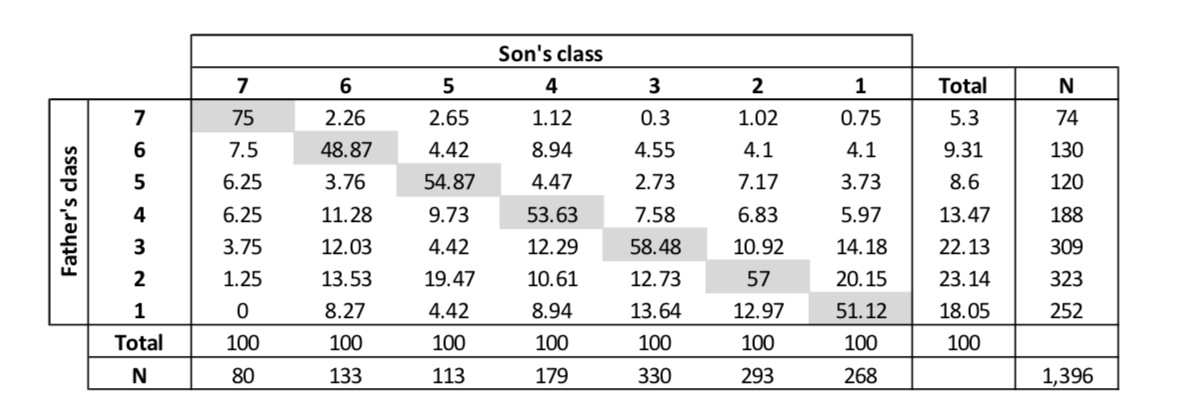
\includegraphics[width=12cm]{table9.png}
    \caption{Inflow mobility, pre‐1750}
 \end{figure}
\end{frame}
%------------------------------------------------
\section{Conclusion}
%------------------------------------------------
\begin{frame}
\frametitle{Conclusion}    
As conclusion the paper offer the suggestion that the spread of the middle class values to lower social classes, through social mobility, might have been a stimulus to England’s industrial revolution by testing:\\~\\
 \begin{itemize}
    \item The middle class families were more successful in terms of reproduction than their lower social‐class counterparts
    \item The pre‐industrial England was socially static over time. According to the Cambridge data
  \end{itemize}\\~\\
 As both analysis were true we can construed that the suggestion were true

\end{frame}
%------------------------------------------------
\section{References}
%------------------------------------------------
% Only use if you do not have bib file
% Otherwise use other option
\begin{frame}
\frametitle{References}
\footnotesize{
\begin{thebibliography}{99} % Beamer does not support BibTeX so references must be inserted manually as below
\bibitem[Clark; Cummins, 2010]{p1} Clark et al. (2010)
\newblock Malthus to modernity: England’s first
fertility transition
\newblock \emph{Mimeo}
\end{thebibliography}
}
\footnotesize{
\begin{thebibliography}{99} % Beamer does not support BibTeX so references must be inserted manually as below
\bibitem[BOBERG-FAZLIC et al, 2011]{p1} Boberg-Fazlic et al. (2011)
\newblock Survival of the richest? Social status, fertility and social mobility in England 1541-1824
\newblock \emph{European Review of Economic History}
\end{thebibliography}
}
\footnotesize{
\begin{thebibliography}{99} % Beamer does not support BibTeX so references must be inserted manually as below
\bibitem[Wrigley et al, 1997]{p1}  Wrigley et all. (1997)
\newblock English Population History from Family
\end{thebibliography}
}
\end{frame}

% bib file based references
%\begin{frame}[allowframebreaks]{References}
%\def\newblock{}
%\bibliographystyle{econometrica}
%\bibliography{bibfile}
%\end{frame}

%------------------------------------------------
\section{Contact information}
%------------------------------------------------
% Only use if you do not have bib file
% Otherwise use other option
\begin{frame}
\frametitle{Contact information}

María Paula Castañeda León - castanedamaria@javeriana.edu.co

Hernando Valentín Padilla - padilla.hernando@javeriana.edu.co

\end{frame}


% bib file based references
%\begin{frame}[allowframebreaks]{References}
%\def\newblock{}
%\bibliographystyle{econometrica}
%\bibliography{bibfile}
%\end{frame}

%------------------------------------------------
\begin{frame}
\Huge{\centerline{The End}}
\end{frame}

%----------------------------------------------------------------------------------------

\end{document} 